\marginnote{
	\begin{minipage}{5.5cm}
		\begin{figure}[H]\centering
	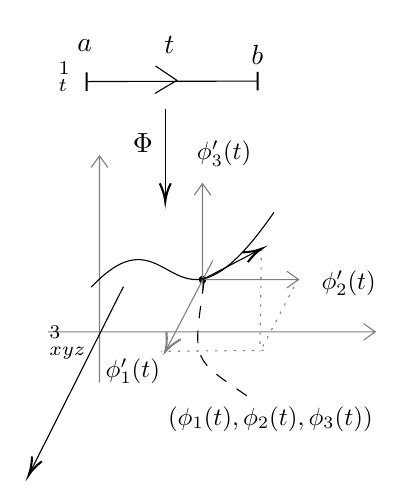
\begin{tikzpicture}[x=0.6pt,y=0.6pt,yscale=-1,xscale=1]
	%uncomment if require: \path (0,439); %set diagram left start at 0, and has height of 439
	
	%Straight Lines [id:da010258542781164337] 
	\draw    (142.15,171.48) -- (39.14,171.77) ;
	\draw [shift={(39.14,171.77)}, rotate = 359.83000000000004] [color={rgb, 255:red, 0; green, 0; blue, 0 }  ][line width=0.75]    (0,5.59) -- (0,-5.59)   ;
	\draw [shift={(142.15,171.48)}, rotate = 359.83000000000004] [color={rgb, 255:red, 0; green, 0; blue, 0 }  ][line width=0.75]    (0,5.59) -- (0,-5.59)   ;
	\draw   (80.67,162.39) -- (93.51,171.04) -- (80.22,178.97) ;
	
	%Shape: Axis 2D [id:dp6889745385829058] 
	\draw [color={rgb, 255:red, 128; green, 128; blue, 128 }  ,draw opacity=1 ] (16,322.5) -- (212.93,322.5)(46.93,216.5) -- (46.93,353.04) (205.93,317.5) -- (212.93,322.5) -- (205.93,327.5) (41.93,223.5) -- (46.93,216.5) -- (51.93,223.5)  ;
	%Shape: Boxed Line [id:dp16438192577140776] 
	\draw    (61.33,295.28) -- (5.18,407.02) ;
	\draw [shift={(4.28,408.8)}, rotate = 296.68] [color={rgb, 255:red, 0; green, 0; blue, 0 }  ][line width=0.75]    (10.93,-3.29) .. controls (6.95,-1.4) and (3.31,-0.3) .. (0,0) .. controls (3.31,0.3) and (6.95,1.4) .. (10.93,3.29)   ;
	
	%Shape: Circle [id:dp7087171813046038] 
	\draw  [fill={rgb, 255:red, 0; green, 0; blue, 0 }  ,fill opacity=1 ] (110.93,291.03) .. controls (110.93,289.95) and (110.05,289.07) .. (108.97,289.07) .. controls (107.88,289.07) and (107,289.95) .. (107,291.03) .. controls (107,292.12) and (107.88,293) .. (108.97,293) .. controls (110.05,293) and (110.93,292.12) .. (110.93,291.03) -- cycle ;
	%Shape: Axis 2D [id:dp3359608795022041] 
	\draw [color={rgb, 255:red, 128; green, 128; blue, 128 }  ,draw opacity=1 ] (102.54,291.03) -- (166.79,291.03)(108.97,233.21) -- (108.97,297.46) (159.79,286.03) -- (166.79,291.03) -- (159.79,296.03) (103.97,240.21) -- (108.97,233.21) -- (113.97,240.21)  ;
	%Straight Lines [id:da9864853885071442] 
	\draw [color={rgb, 255:red, 128; green, 128; blue, 128 }  ,draw opacity=1 ]   (115.15,279.5) -- (87.41,332.66) ;
	\draw [shift={(86.48,334.43)}, rotate = 297.56] [color={rgb, 255:red, 128; green, 128; blue, 128 }  ,draw opacity=1 ][line width=0.75]    (10.93,-4.9) .. controls (6.95,-2.3) and (3.31,-0.67) .. (0,0) .. controls (3.31,0.67) and (6.95,2.3) .. (10.93,4.9)   ;
	
	%Shape: Boxed Line [id:dp9016333005766098] 
	\draw [color={rgb, 255:red, 128; green, 128; blue, 128 }  ,draw opacity=1 ] [dash pattern={on 0.84pt off 2.51pt}]  (166.59,290.5) -- (143.48,334.77) ;
	
	
	%Shape: Boxed Line [id:dp3804166141611265] 
	\draw [color={rgb, 255:red, 128; green, 128; blue, 128 }  ,draw opacity=1 ] [dash pattern={on 0.84pt off 2.51pt}]  (145.8,333.67) -- (83.84,334.26) ;
	
	
	%Straight Lines [id:da6259198083466047] 
	\draw [color={rgb, 255:red, 128; green, 128; blue, 128 }  ,draw opacity=1 ] [dash pattern={on 0.84pt off 2.51pt}]  (144.44,272.48) -- (143.48,334.43) ;
	
	
	%Straight Lines [id:da43876051555056905] 
	\draw    (108.97,291.03) -- (142.66,273.4) ;
	\draw [shift={(144.44,272.48)}, rotate = 512.38] [color={rgb, 255:red, 0; green, 0; blue, 0 }  ][line width=0.75]    (10.93,-3.29) .. controls (6.95,-1.4) and (3.31,-0.3) .. (0,0) .. controls (3.31,0.3) and (6.95,1.4) .. (10.93,3.29)   ;
	
	%Curve Lines [id:da9461526898510314] 
	\draw    (41.93,295.6) .. controls (91.93,242.6) and (88.93,341.6) .. (151.93,250.6) ;
	
	
	%Curve Lines [id:da3687316850988571] 
	\draw  [dash pattern={on 4.5pt off 4.5pt}]  (109.93,292.03) .. controls (102.75,343.27) and (101.75,337.27) .. (141.75,365.27) ;
	
	
	%Straight Lines [id:da41758799892896037] 
	\draw    (86.5,188) -- (86.5,242) ;
	\draw [shift={(86.5,244)}, rotate = 270] [color={rgb, 255:red, 0; green, 0; blue, 0 }  ][line width=0.75]    (10.93,-3.29) .. controls (6.95,-1.4) and (3.31,-0.3) .. (0,0) .. controls (3.31,0.3) and (6.95,1.4) .. (10.93,3.29)   ;
	
	
	% Text Node
	\draw (38,150) node   {$a$};
	% Text Node
	\draw (142,156) node   {$b$};
	% Text Node
	\draw (89,150) node   {$t$};
	% Text Node
	\draw (26,169) node   {$\R^{1}_{t}$};
	% Text Node
	\draw (73,209) node   {$\Phi $};
	% Text Node
	\draw (67,346.22) node [scale=0.9]  {$\phi '_{1}( t)$};
	% Text Node
	\draw (197,293.22) node [scale=0.9]  {$\phi '_{2}( t)$};
	% Text Node
	\draw (122,215.22) node [scale=0.9]  {$\phi '_{3}( t)$};
	% Text Node
	\draw (28,329) node   {$\R^{3}_{xyz}$};
	% Text Node
	\draw (149.82,374.97) node [scale=0.9,color={rgb, 255:red, 0; green, 0; blue, 0 }  ,opacity=1 ]  {$( \phi _{1}( t) ,\phi _{2}( t) ,\phi _{3}( t))$};
	
	
	\end{tikzpicture}
	
			\caption{Mapeo del caso 1-3.}\label{ch0d3}
		\end{figure}
\end{minipage}}[-3em]


